\section{PCB Design}
This section describes the PCB design and explains the decisions related to this.
It has several headers for debugging purposes.

\begin{figure}[h]
    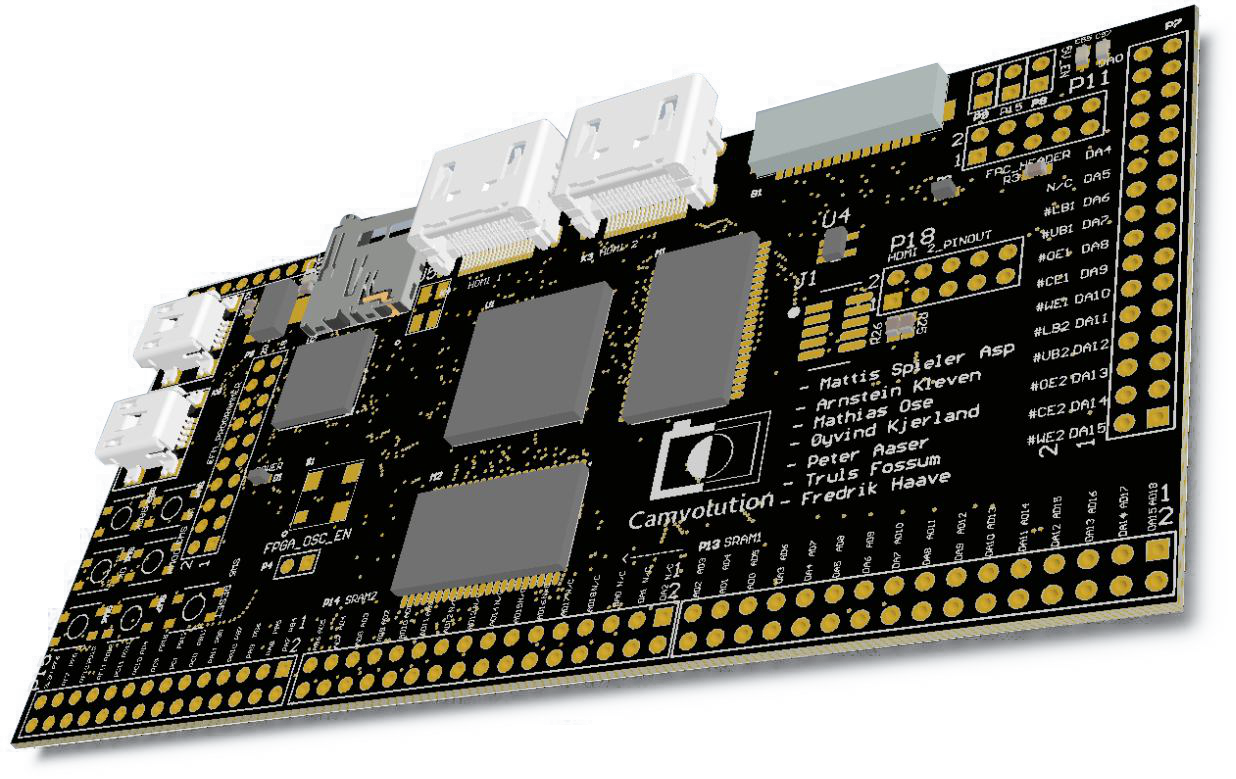
\includegraphics[width=\linewidth]{img/OverviewCamvolutionKit}
    \caption{Camvolution board layout}
\end{figure}

\subsection{Board Features}
Figure \ref{fig:BoardLayout} shows an overview of the board with various components labeled.

\begin{itemize}
    \item Xilinx Spartan-6 FPGA
    \item Silicon Labs EFM32GG MCU
    \item Connectors
        \begin{itemize}
            \item HDMI I/O
            \item FPC Camera
            \item MicroSD
        \end{itemize}
    \item 120MHz Oscillator for FPGA
    \item 48MHz Crystal for MCU
    \item Digital I/O
        \begin{itemize}
            \item 7 Mechanical Buttons
            \item 7 Expansion Headers
            \item 2 LEDs
        \end{itemize}
    \item External memory
        \begin{itemize}
            \item 2 AS7C38098A SRAM
        \end{itemize}
\end{itemize}

\begin{figure}
    \includegraphics[width=\linewidth]{img/"Overview of Camvolution kit".jpg}
    \caption{Overview of Camvolution board}
    \label{fig:BoardLayout}
\end{figure}

\subsection{Power Supply}
The board is powered by a MiniUSB connector, with two possible options for powering it.
It can be connected either to the PC, or to a 5V USB power supply.

The 5V is regulated with a 3.3V low-dropout (LDO) regulator, which gives power to most of the board.
This 3.3V is also connected to a 1.2V LDO regulator which powers the minimum required power pins on the Xilinx Spartan-6 FPGA.

\subsection{Clock Generation}
\subsubsection{FPGA Oscillator}
The oscillator is connected to an enable signal on the MCU.
To enable the 120MHz oscillator, the signal must be set to output and driven high.
The oscillator enable pin is also connected to an external input and can be set high by connecting this pin to VCC.
The easiest way of enabling the oscillator is to add a jumper on the FPGA\_OSC\_EN header.

\subsubsection{MCU External Crystal}
The MCU has one internal and one external clock.
The external clock source is 48MHz.

\subsection{Connectors}
\subsubsection{HDMI}
There are two HDMI connectors on the board.
Both of them must also be connected to 5V, and can be set with a jumper at header 8 and header 15 respectively.
The HDMI 2 is also connected to header P18, this can be used for debugging.
See Table \ref{HDMI_Connector} for pinouts.

\subsubsection{FPC Camera Connector}
There is one Raspberry Pi camera connector on the board.
It is also connected to header P11.
This and can be used for debugging.
See Figure \ref{fig:FpcHeader} for pin configuration.

\subsection{Digital I/O}
\subsubsection{Buttons}
The board contains seven buttons.
When the button is pushed down, the input pin will be grounded.

The FPGA has two buttons for control, and the MCU has four buttons for control.
See Table \ref{tab:Buttons} for info.
The last buttons is connected to reset on the MCU.

\subsubsection{Header Output}
The MCU has spare pins that all are available on the P15 header pins.
Pin 28 on P15 header is 3.3V VCC.
See Table \ref{tab:HeaderOut} for location of pins.

\subsection{SRAM}
\label{subsec:sram}
The FPGA is connected to two SRAM chips from Alliance Memory, one on bank 1 and another on bank 2.
They support a data width of 16 bits and have an access time of \unit[10]{ns} \cite{sramdatasheet}, which means we have a maximum throughput of $(\unit[10]{ns})^{-1} = \unit[1,6]{Gbps}$ to each chip.
This is more than sufficient for our application as can be seen in Table \ref{tab:BitRates}.

To make debugging easier, all wires connecting the FPGA and SRAM chips have been placed on headers.

\subsection{JTAG}
Both the FPGA and the MCU is connected to a JTAG header.
The MCU is connected to a 20 pin JTAG header that can be used with the generic programming header from the MCU development kit.
The FPGA is connected to a 8 pin JTAG header. This can be routed to a debugger used for FPGA programming.
See Table \ref{tab:EfmProgrammer} for MCU JTAG header, see Figure \ref{fig:FpgaProgrammer} for FPGA JTAG header.

\begin{table}[]
    \centering
    \begin{tabular}{ll}
        Pin                     & USAGE     \\
        \hline
        1                       & VCC       \\
        3                       & N/C       \\
        5                       & N/C       \\
        7                       & CS / PF0  \\
        9                       & CLK / PF1 \\
        11                      & N/C       \\
        13                      & PF2       \\
        15                      & RESET     \\
        17                      & N/C       \\
        19                      & N/C       \\
        4,6,8,10,12,14,16,18,20 & GND       \\
        2                       & N/C
    \end{tabular}
    \caption{Programming Output for MCU}
    \label{tab:EfmProgrammer}
\end{table}

\begin{figure}
    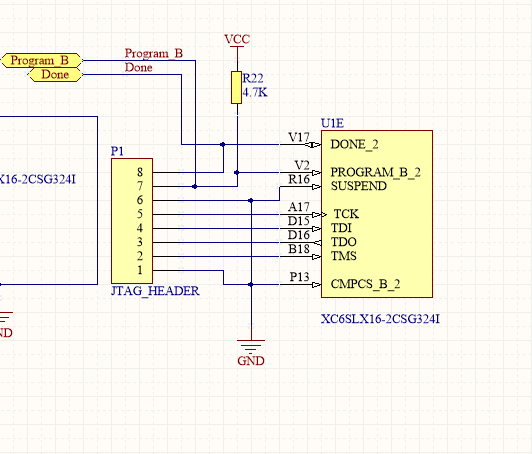
\includegraphics[width=\linewidth]{img/FPGA_Programmer}
    \caption{Programming output for FPGA}
    \label{fig:FpgaProgrammer}
\end{figure}

\subsection{Programming FPGA Using MCU SPI}
The FPGA can also be programmed using SPI from the MCU.
INIT\_B shares the same pin as the SRAM2 data line, but when programming the FPGA the SRAM will not be active.
See Table \ref{tab:SpiProgrammer}.

\begin{table}[]
    \centering
    \begin{tabular}{lll}
        MCU pin & FPGA & Usage   \\
        \hline
        PB8     & U3   & INIT\_B \\
        PD3     & U15  & CS      \\
        PD2     & R15  & CLK     \\
        PD1     & V16  & RX      \\
        PD0     & R13  & TX
    \end{tabular}
    \caption{Programming FPGA using MCU SPI}
    \label{tab:SpiProgrammer}
\end{table}

\subsection{LED}
There are two LEDs on the board.
One is connected to power on the board and will light up if power is connected.
The last LED is programmable from the FPGA.

\subsection{EBI Bus}
The FPGA and the MCU is connected with a high speed External Bus Interface (EBI) bus with 20 addressable pins and 16 data lines.
See Appendix \ref{app:pinouts}, Figure \ref{fig:EbiBus} and \ref{fig:EbiControl} for EBI bus.

\subsection{List of Components}
See Table \ref{listofcomponents} in Appendix \ref{app:components} for a list of components used on the board.
